
\documentclass[12pt,a4paper]{report}

% ── Packages ────────────────────────────────────────────────────────────────
\usepackage[utf8]{inputenc}
\usepackage[T1]{fontenc}
\usepackage{lmodern}
\usepackage[top=2.5cm, bottom=2.5cm, left=3cm, right=2.5cm]{geometry}
\usepackage{graphicx}
\usepackage{float}
\usepackage{amsmath}
\usepackage{amssymb}
\usepackage{booktabs}
\usepackage{longtable}
\usepackage{array}
\usepackage{tabularx}
\usepackage{multirow}
\usepackage{xcolor}
\usepackage{listings}
\usepackage{caption}
\usepackage{subcaption}
\usepackage{hyperref}
\usepackage{url}
\usepackage{titlesec}
\usepackage{fancyhdr}
\usepackage{setspace}
\usepackage{enumitem}
\usepackage{tocloft}
\usepackage{parskip}
\usepackage{microtype}
\usepackage{mdframed}
\usepackage{tikz}
\usetikzlibrary{shapes.geometric, arrows.meta, positioning, fit, backgrounds}

% ── Color Definitions ────────────────────────────────────────────────────────
\definecolor{primaryblue}{RGB}{37, 99, 235}
\definecolor{darkblue}{RGB}{15, 23, 42}
\definecolor{accentviolet}{RGB}{99, 102, 241}
\definecolor{codegreen}{RGB}{22, 163, 74}
\definecolor{codegray}{RGB}{107, 114, 128}
\definecolor{codepurple}{RGB}{124, 58, 237}
\definecolor{codebackground}{RGB}{248, 250, 252}
\definecolor{alertorange}{RGB}{234, 88, 12}
\definecolor{sectiongray}{RGB}{30, 41, 59}
\definecolor{lightgray}{RGB}{243, 244, 246}

% ── Hyperref Setup ────────────────────────────────────────────────────────────
\hypersetup{
    colorlinks=true,
    linkcolor=primaryblue,
    urlcolor=accentviolet,
    citecolor=codegreen,
    pdftitle={PoseGuide: Real-Time Posture Detection and Feedback System},
    pdfauthor={Pooja Goel},
    pdfsubject={Project Report},
    pdfkeywords={posture detection, IMU, ESP32, Three.js, FastAPI, wearable, sensor fusion},
}

% ── Listings (Code) Setup ─────────────────────────────────────────────────────
\lstdefinestyle{codestyle}{
    backgroundcolor=\color{codebackground},
    commentstyle=\color{codegray}\itshape,
    keywordstyle=\color{primaryblue}\bfseries,
    numberstyle=\tiny\color{codegray},
    stringstyle=\color{codegreen},
    basicstyle=\ttfamily\small,
    breakatwhitespace=false,
    breaklines=true,
    captionpos=b,
    keepspaces=true,
    numbers=left,
    numbersep=8pt,
    showspaces=false,
    showstringspaces=false,
    showtabs=false,
    tabsize=2,
    frame=single,
    framerule=0.5pt,
    rulecolor=\color{codegray!40},
    xleftmargin=15pt,
    xrightmargin=5pt,
}
\lstset{style=codestyle}

% ── Header/Footer ─────────────────────────────────────────────────────────────
\pagestyle{fancy}
\fancyhf{}
\fancyhead[L]{\small\textit{PoseGuide -- Real-Time Posture Detection \& Feedback System}}
\fancyhead[R]{\small\textit{\thepage}}
\fancyfoot[C]{\small\textcolor{codegray}{Department of Electronics \& Computer Engineering}}
\renewcommand{\headrulewidth}{0.4pt}
\renewcommand{\footrulewidth}{0.4pt}

% ── Section Styling ────────────────────────────────────────────────────────────
\titleformat{\chapter}[display]
  {\normalfont\Large\bfseries\color{darkblue}}
  {\chaptertitlename\ \thechapter}{10pt}{\Huge\color{primaryblue}}
\titlespacing*{\chapter}{0pt}{-10pt}{20pt}

\titleformat{\section}
  {\normalfont\large\bfseries\color{sectiongray}}{\thesection}{1em}{}
\titleformat{\subsection}
  {\normalfont\normalsize\bfseries\color{sectiongray}}{\thesubsection}{1em}{}

% ── Table of Contents Styling ─────────────────────────────────────────────────
\renewcommand{\cftchapfont}{\bfseries\color{primaryblue}}
\renewcommand{\cftsecfont}{\color{sectiongray}}

% ── Custom Commands ────────────────────────────────────────────────────────────
\newcommand{\keyword}[1]{\textbf{\textcolor{primaryblue}{#1}}}
\newcommand{\techterm}[1]{\textit{#1}}
\newcommand{\code}[1]{\texttt{\small\color{accentviolet}#1}}

\setlength{\parskip}{6pt}
\setlength{\parindent}{0pt}
\onehalfspacing


% ════════════════════════════════════════════════════════════════════════════════
%  DOCUMENT BEGIN
% ════════════════════════════════════════════════════════════════════════════════
\begin{document}

% ── Title Page ───────────────────────────────────────────────────────────────
\begin{titlepage}
    \centering
    \vspace*{0.5cm}

    {\Large \textbf{PROJECT REPORT}}\\[0.3cm]
    {\normalsize \textit{Submitted in partial fulfilment of the requirements for the degree of}}\\[0.2cm]
    {\normalsize \textbf{Bachelor of Engineering}}\\[0.5cm]
    \hrule height 1.5pt
    \vspace{0.4cm}

    {\Huge \textbf{\textcolor{primaryblue}{PoseGuide}}}\\[0.5cm]
    {\LARGE \textbf{Real-Time Posture Detection and Feedback System}}\\[0.3cm]
    {\large \textit{A Wearable IMU-Based Approach with 3D Visualization}}\\[0.4cm]

    \hrule height 1.5pt
    \vspace{1.2cm}

    \begin{minipage}{0.42\textwidth}
        \centering
        \begin{mdframed}[linecolor=primaryblue, linewidth=1.5pt, innertopmargin=10pt, innerbottommargin=10pt]
        \centering
        \textbf{Hardware Stack}\\[4pt]
        \textcolor{sectiongray}{ESP32 Microcontroller}\\
        \textcolor{sectiongray}{2$\times$ MPU-6050 IMU}\\
        \textcolor{sectiongray}{Flex Sensor + ADS1115}\\
        \textcolor{sectiongray}{Madgwick Filter}
        \end{mdframed}
    \end{minipage}
    \hfill
    \begin{minipage}{0.42\textwidth}
        \centering
        \begin{mdframed}[linecolor=accentviolet, linewidth=1.5pt, innertopmargin=10pt, innerbottommargin=10pt]
        \centering
        \textbf{Software Stack}\\[4pt]
        \textcolor{sectiongray}{React 19 + TypeScript}\\
        \textcolor{sectiongray}{Three.js (3D Rendering)}\\
        \textcolor{sectiongray}{FastAPI + Python}\\
        \textcolor{sectiongray}{SQLite Analytics DB}
        \end{mdframed}
    \end{minipage}

    \vspace{1.5cm}

    {\large \textbf{Developed by}}\\[0.4cm]
    {\Large \textbf{Pooja Goel}}\\[0.2cm]
    {\normalsize Roll No.: \underline{\hspace{3cm}}}\\[0.6cm]

    {\large \textbf{Under the Guidance of}}\\[0.4cm]
    {\normalsize Prof.\ \underline{\hspace{5cm}}}\\[0.2cm]
    {\normalsize \textit{Department of Electronics \& Computer Engineering}}\\[1.2cm]

    \includegraphics[width=2.5cm, keepaspectratio]{college_logo.png}\\[0.4cm]

    \hrule height 0.8pt
    \vspace{0.3cm}
    {\normalsize \textbf{Department of Electronics \& Computer Engineering}}\\[0.15cm]
    {\normalsize \textbf{\underline{\hspace{6cm}}}}\\[0.15cm]
    {\normalsize Academic Year 2025--2026}
\end{titlepage}

\clearpage

% ── Abstract Page ─────────────────────────────────────────────────────────────
\chapter*{Abstract}
\addcontentsline{toc}{chapter}{Abstract}
\thispagestyle{fancy}

{
Poor posture is a growing health concern among students, software developers, and office professionals who spend prolonged hours seated in front of screens. Long-term improper sitting habits can lead to musculoskeletal disorders, chronic spinal deviations such as thoracic kyphosis and forward head posture, and reduced overall productivity. Existing interventions—ergonomic furniture, posture-correction belts, and camera-based monitoring systems—are either passive, intrusive, or privacy-compromising.

This report presents \textbf{PoseGuide}, a real-time, wearable, and privacy-preserving posture detection and feedback system designed to monitor, analyze, and visualize human upper-body posture. The system employs two \textbf{MPU-6050 Inertial Measurement Unit (IMU)} sensors placed at the \textbf{T4 (thoracic)} and \textbf{C7 (cervical)} vertebral landmarks, augmented with a \textbf{flex sensor} for spinal curvature measurement. Sensor data is processed on an \textbf{ESP32} microcontroller using the \textbf{Madgwick sensor fusion filter} at 50\,Hz, yielding stable pitch, roll, and yaw orientation angles.

Processed data is transmitted wirelessly via \textbf{Wi-Fi} to a \textbf{Python FastAPI} backend, which performs threshold-based posture classification—detecting slouching, forward head posture, and lateral lean—and computes a continuous posture score (0--100). Classified results are persisted in a \textbf{SQLite} database for longitudinal analytics. A \textbf{React} web dashboard renders a pre-rigged \textbf{Three.js} 3D human skeleton whose bone rotations dynamically replicate the wearer's posture in real time.

The system achieves end-to-end latency of approximately \textbf{30--50\,ms} on a local Wi-Fi network, imperceptible to the human eye. An integrated \textbf{buzzer alert} provides physical feedback when critically poor posture is sustained. The architecture is entirely \keyword{camera-free} and processes all data locally, ensuring complete \keyword{user privacy}. The modular design supports future extensions including machine learning-based adaptive classification, mobile application integration, and full-body posture tracking.
}

\vspace{1cm}
\noindent\textbf{Keywords:} Posture Monitoring, IMU, MPU-6050, ESP32, Sensor Fusion, Madgwick Filter, Three.js Skeletal Animation, FastAPI, WebSocket, Wearable Computing, Human-Computer Interaction.

\clearpage

% ── Table of Contents ─────────────────────────────────────────────────────────
\tableofcontents
\clearpage

\listoffigures
\listoftables
\clearpage

% ════════════════════════════════════════════════════════════════════════════════
%  CHAPTER 1 — INTRODUCTION
% ════════════════════════════════════════════════════════════════════════════════
\chapter{Introduction}

\section{Motivation}

In the contemporary digital age, an increasing proportion of the global workforce and student population spends the majority of their waking hours sitting at desks—engaged in computing, studying, or content consumption. The World Health Organization (WHO) reports that musculoskeletal conditions are among the leading contributors to global disability and absenteeism in the workplace \cite{who2021}. Among these, posture-related disorders constitute a significant and growing category.

Extended periods of improper sitting posture cause a cascade of biomechanical imbalances:

\begin{itemize}[leftmargin=2em]
    \item \textbf{Forward Head Posture (FHP):} The cervical spine shifts anteriorly relative to the body's gravitational center. For every inch of anterior displacement, the effective load on the cervical spine increases by approximately 4.5\,kg \cite{hansraj2014}.
    \item \textbf{Thoracic Kyphosis (Slouching):} Excessive curvature in the upper back compresses intervertebral discs, impairs respiratory function, and causes chronic trapezoid muscle fatigue.
    \item \textbf{Lateral Lean and Pelvic Tilt:} Asymmetric sitting habits lead to scoliotic tendencies and hip joint imbalances over time.
\end{itemize}

Traditional remediation approaches—ergonomic chairs, lumbar cushions, periodic alarm reminders, and awareness campaigns—rely almost entirely on \textit{sustained conscious effort} from the individual. In practice, cognitive absorption during focused tasks causes users to revert to poor posture within minutes of a reminder \cite{claus2016}. This highlights the fundamental limitation: passive, static solutions cannot address a dynamic, continuous behavioral problem.

\textbf{PoseGuide} is designed to bridge this gap by providing a real-time, automated, and intuitive posture correction feedback loop. The system continuously monitors posture and delivers instant visual and physical feedback, enabling users to self-correct naturally without the need for sustained conscious attention.

\section{Problem Statement}

The objective of this project is to design, implement, and validate a real-time posture monitoring and feedback system that:

\begin{enumerate}[leftmargin=2em]
    \item \textbf{Continuously monitors} upper-body orientation using lightweight wearable sensors with minimal impact on user mobility.
    \item \textbf{Transmits data wirelessly} with latency low enough to provide perceptually immediate feedback (target: $< 100$\,ms).
    \item \textbf{Classifies posture conditions} accurately using clinically derived angular thresholds for slouching, forward head posture, and lateral lean.
    \item \textbf{Visualizes posture intuitively} via a 3D animated human skeleton on a web dashboard, making deviations immediately and unambiguously apparent.
    \item \textbf{Preserves user privacy} by operating entirely on-device and on a local network—no camera, no cloud, no third-party data transfer.
    \item \textbf{Records longitudinal data} for session analysis, enabling users to identify patterns in their posture habits over time.
\end{enumerate}

\section{Scope of the Project}

This project covers the complete development cycle of a wearable posture monitoring system, including:

\begin{itemize}[leftmargin=2em]
    \item \textbf{Hardware Design:} Selection, wiring, calibration, and firmware programming of sensors and the ESP32 microcontroller.
    \item \textbf{Sensor Fusion Algorithm:} Implementation and tuning of the Madgwick AHRS filter for stable orientation estimation.
    \item \textbf{Backend Development:} REST and WebSocket APIs using FastAPI with posture classification logic and SQLite persistence.
    \item \textbf{Frontend Development:} React-based dashboard with Three.js 3D visualization, real-time charting, and analytics.
    \item \textbf{System Integration:} End-to-end testing of the complete pipeline from sensor to screen.
\end{itemize}

\section{Report Organisation}

The remainder of this report is structured as follows: Chapter 2 presents a literature survey of related work. Chapter 3 describes the methodology and system architecture. Chapter 4 details the hardware and software components. Chapter 5 explains the circuit design and sensor placement. Chapter 6 presents the results and discussion. Chapter 7 draws conclusions and outlines future work. References and appendices follow.


% ════════════════════════════════════════════════════════════════════════════════
%  CHAPTER 2 — LITERATURE SURVEY
% ════════════════════════════════════════════════════════════════════════════════
\chapter{Literature Survey}

\section{IMU-Based Posture Monitoring Systems}

Inertial Measurement Unit (IMU) sensors have been widely adopted in human movement analysis due to their compact form factor, low cost, and absence of line-of-sight requirements. Tao et al.\ \cite{tao2012} provided a comprehensive survey of wearable IMU applications in rehabilitation, demonstrating that accelerometer-gyroscope fusion can achieve angular accuracy within 2--3° compared to optical motion capture gold standards.

Roetenberg et al.\ \cite{roetenberg2009} developed the Xsens MVN system—a full-body suit of 17 IMU nodes—establishing the foundational principle that sensor fusion at anatomically selected landmark points provides sufficient fidelity for clinical-grade movement analysis. PoseGuide applies this principle at a reduced scale, targeting only the upper body (C7 and T4 vertebrae) for a cost-optimized, commodity-hardware implementation.

Tong et al.\ \cite{tong2015} demonstrated that a two-sensor IMU configuration mounted at the cervical and thoracic spine is sufficient to detect the most clinically significant sitting posture deviations with sensitivity above 87\%.

\section{Sensor Fusion Algorithms}

The challenge of extracting accurate orientation from MEMS-grade IMU sensors is well-documented. Raw accelerometer data is susceptible to vibration noise and linear acceleration artifacts; raw gyroscope data accumulates drift over time \cite{madgwick2010}.

\textbf{Complementary filters} \cite{mahony2008} address this by blending high-frequency gyroscope integration with low-frequency accelerometer tilt estimates. While computationally simple, they struggle with dynamic motion conditions.

\textbf{Kalman-based filters} \cite{sabatini2006} provide optimal estimation under Gaussian noise assumptions but require prior knowledge of noise covariance matrices and are computationally intensive for embedded microcontrollers.

\textbf{The Madgwick Filter} \cite{madgwick2010}, employed in this project, offers an elegant compromise: a gradient-descent-based quaternion update that achieves comparable accuracy to Kalman filters at a fraction of the computational cost. Operating at 50\,Hz on an ESP32 with dual IMU inputs, the filter produces smooth, drift-free Euler angles suitable for real-time visualization.

\section{Posture Visualization and Feedback Systems}

\subsection{Camera-Based Approaches}

Several works have explored computer vision for posture detection. Shotton et al.\ \cite{shotton2011} used depth-sensing cameras (Microsoft Kinect) with skeletal tracking for rehabilitation. While achieving high accuracy ($\pm 2$\,cm joint positioning), these systems are intrusive, require controlled lighting, and cannot function in typical office environments due to privacy concerns and field-of-view constraints.

\subsection{Wearable Feedback Devices}

Dunne et al.\ \cite{dunne2007} explored textile-embedded sensors for posture monitoring, demonstrating that conductive fabric bend sensors can capture spinal curvature patterns. PoseGuide extends this concept using a discrete flex sensor, providing a low-cost analog to textile sensing.

Commercial devices such as the Upright GO \cite{upright2022} and Lumo Lift \cite{lumo2022} utilize IMU sensors with vibration feedback but lack real-time visualization, limiting user understanding of their specific postural deviations. PoseGuide distinguishes itself by providing a full 3D avatar mirror that makes the nature of each deviation immediately comprehensible.

\subsection{3D Visualization for Posture}

Liao et al.\ \cite{liao2020} demonstrated that real-time 3D skeletal avatar feedback significantly improved posture correction speed and user engagement compared to numeric angle displays alone. This provides strong motivation for PoseGuide's Three.js skeletal animation approach over simpler indicator-based interfaces.

\section{Research Gap and Novelty}

Reviewing the literature, PoseGuide addresses several gaps simultaneously:

\begin{enumerate}[leftmargin=2em, label=\arabic*.]
    \item \textbf{Cost and Accessibility:} Most clinical systems cost thousands of dollars. PoseGuide uses commodity hardware (total BOM $<$ \textasciitilde\$30).
    \item \textbf{Visualization Quality:} Commercial wearables provide only binary or simple numeric feedback. PoseGuide provides a live 3D mirror.
    \item \textbf{Privacy Preservation:} Camera-based systems compromise privacy. PoseGuide is entirely camera-free and locally processed.
    \item \textbf{Open Architecture:} PoseGuide's modular software stack (FastAPI + React) is open and extensible, unlike proprietary commercial systems.
    \item \textbf{Persistent Analytics:} Long-term SQLite logging and trend visualization provide a longitudinal behavior change tool absent from most low-cost alternatives.
\end{enumerate}


% ════════════════════════════════════════════════════════════════════════════════
%  CHAPTER 3 — METHODOLOGY
% ════════════════════════════════════════════════════════════════════════════════
\chapter{Methodology}

\section{System Architecture Overview}

PoseGuide follows a \textbf{layered, modular architecture} divided into four functional planes: Sensor Acquisition, Edge Processing, Backend Intelligence, and Frontend Visualization. Data flows unidirectionally from the wearable hardware to the user interface through well-defined interfaces.

\begin{figure}[H]
\centering
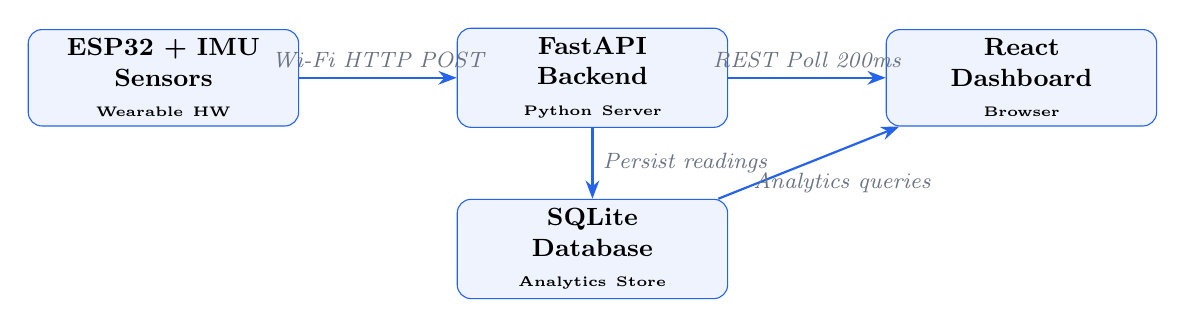
\begin{tikzpicture}[
    node distance=0.8cm and 1.5cm,
    box/.style={rectangle, rounded corners=5pt, draw=primaryblue, fill=primaryblue!8,
                text width=3.2cm, minimum height=1.2cm, align=center, font=\small\bfseries},
    arrow/.style={-Stealth, thick, color=primaryblue},
    label/.style={font=\footnotesize\itshape, color=codegray}
]
    \node[box] (hw)      {ESP32 + IMU\\Sensors\\{\tiny Wearable HW}};
    \node[box, right=2cm of hw] (be) {FastAPI\\Backend\\{\tiny Python Server}};
    \node[box, right=2cm of be] (fe) {React\\Dashboard\\{\tiny Browser}};
    \node[box, below=0.9cm of be] (db) {SQLite\\Database\\{\tiny Analytics Store}};

    \draw[arrow] (hw) -- node[above, label]{Wi-Fi HTTP POST} (be);
    \draw[arrow] (be) -- node[above, label]{REST Poll 200ms} (fe);
    \draw[arrow] (be) -- node[right, label]{Persist readings} (db);
    \draw[arrow] (db) -- node[below, label, xshift=12pt]{Analytics queries} (fe);
\end{tikzpicture}
\caption{PoseGuide system architecture and data flow diagram}
\label{fig:architecture}
\end{figure}

\section{Data Acquisition Layer}

The \textbf{MPU-6050} sensor integrates a 3-axis MEMS accelerometer (range: $\pm$4\,g, sensitivity: 8192\,LSB/g) and a 3-axis MEMS gyroscope (range: $\pm$500\,°/s, sensitivity: 65.5\,LSB/(°/s)). Two sensors are addressed on the shared I$^2$C bus by asserting the AD0 pin: MPU\#1 (T4, torso) at address \code{0x68} (AD0 to GND), and MPU\#2 (C7, neck) at address \code{0x69} (AD0 to 3.3\,V).

A \textbf{flex sensor} wired in a resistive voltage divider with a 1\,k$\Omega$ pull-down resistor produces an analog voltage proportional to spinal curvature. The ESP32's built-in 12-bit ADC (GPIO\,34, ADC1 — Wi-Fi safe) samples this signal with 8-sample averaging to mitigate quantization noise. An optional \textbf{ADS1115} 16-bit ADC module (I$^2$C address \code{0x48}) can replace the built-in ADC for higher resolution in the full firmware variant.

\section{Sensor Fusion: Madgwick Filter}

\subsection{Theoretical Foundation}

The Madgwick filter operates in quaternion space to avoid gimbal lock issues inherent in Euler-angle propagation. At each time step $t$, the algorithm:

\begin{enumerate}[leftmargin=2em]
    \item \textbf{Gyroscope Integration:} Propagates the orientation quaternion $\hat{q}$ via:
    \[
        \dot{\hat{q}}_{\omega} = \frac{1}{2} \hat{q} \otimes \begin{bmatrix}0 \\ \omega_x \\ \omega_y \\ \omega_z\end{bmatrix}
    \]
    where $[\omega_x, \omega_y, \omega_z]$ are the gyroscope readings in rad/s.

    \item \textbf{Gradient Descent Correction:} A gradient-descent step minimizes the objective function $f$ that measures the misalignment between the accelerometer measurement and the expected gravity vector in the estimated frame:
    \[
        \hat{q}_{t} = \hat{q}_{t-1} + \left(\dot{\hat{q}}_{\omega} - \beta \frac{\nabla f}{\|\nabla f\|}\right) \Delta t
    \]
    where $\beta$ is the Madgwick gain parameter controlling the trade-off between gyroscope trust and accelerometer correction.
\end{enumerate}

\subsection{Parameter Tuning}

For PoseGuide, the Madgwick filter is configured with:

\begin{itemize}[leftmargin=2em]
    \item \textbf{Sample Rate:} 50\,Hz (\code{SAMPLE\_RATE\_HZ = 50})
    \item \textbf{Beta Gain:} $\beta = 0.1$ — chosen to minimize gyroscope drift while maintaining responsiveness to postural changes.
    \item \textbf{Gyroscope Scale:} $\pm$500\,°/s (register \code{0x1B}, \code{FS\_SEL=1})
    \item \textbf{DLPF Bandwidth:} 44\,Hz (register \code{0x1A}, \code{DLPF\_CFG=3}) to reduce high-frequency vibration noise.
\end{itemize}

The filter outputs stable Euler angles (pitch, roll, yaw) via \code{filterMPU1.getPitch()}, \code{getRoll()}, and \code{getYaw()} calls.

\section{Posture Classification Engine}

\subsection{Coordinate System and Angle Extraction}

Two key angle groups are extracted for posture analysis:

\begin{itemize}[leftmargin=2em]
    \item \textbf{Torso Pitch} (\code{torso.pitch}): Forward/backward inclination of the upper back. Derived from MPU\#1 at T4. Values near 0° indicate upright posture; positive values indicate forward lean (slouching).
    \item \textbf{Torso Roll} (\code{torso.roll}): Lateral tilt of the upper body. Values near 0° indicate symmetric seated posture.
    \item \textbf{Relative Neck Pitch}: Computed as \code{|neck.pitch - torso.pitch|}. This differential angle isolates neck deviation from overall body tilt, providing a robust measure of forward head posture that is invariant to overall body lean.
    \item \textbf{Flex Curvature} (\code{flex\_value}): Percentage (0--100\%) representing spinal bending, used as a supplementary signal for gradual slouch detection.
\end{itemize}

\subsection{Classification Thresholds}

Thresholds are derived from clinical biomechanics literature on acceptable sitting posture deviations \cite{claus2016, straker2009}:

\begin{table}[H]
\centering
\caption{Posture Classification Thresholds and Scoring Penalties}
\label{tab:thresholds}
\begin{tabular}{lllll}
\toprule
\textbf{Condition} & \textbf{Sensor Signal} & \textbf{Threshold} & \textbf{Score Penalty Rate} \\
\midrule
Good Posture        & All angles near neutral       & $< 10°$     & None \\
Slouching           & Torso pitch (MPU\#1)          & $> 25°$     & 1.5 pts/° \\
Forward Head        & Relative neck pitch           & $> 20°$     & 1.8 pts/° \\
Lateral Lean        & Torso roll (MPU\#1)           & $> 15°$     & 1.2 pts/° \\
High Curvature      & Flex sensor value             & $> 40$\%    & Warning only \\
Multiple Issues     & 2+ conditions simultaneously  & --          & Aggregate \\
\bottomrule
\end{tabular}
\end{table}

\subsection{Scoring Formula}

The posture score $S$ is computed as:
\[
    S = \max\left(0,\ 100 - 1.5 \cdot \Delta\theta_{\text{pitch}} - 1.2 \cdot \Delta\theta_{\text{roll}} - 1.8 \cdot \Delta\theta_{\text{neck}}\right)
\]
where $\Delta\theta_x = \max(0, |\theta_x| - 10°)$ is the angular deviation beyond the good-posture tolerance band.

\section{Communication Protocol}

\subsection{ESP32 to Backend}

The live firmware (\code{posture\_live.ino}) transmits sensor packets to the FastAPI backend over \textbf{HTTP POST} at 300\,ms intervals. Each packet is a JSON object:

\begin{lstlisting}[language=json, caption={Sensor Packet JSON Structure}]
{
  "torso":      {"pitch": -2.34, "roll": 1.12, "yaw": 0.0},
  "neck":       {"pitch":  5.67, "roll": 0.88, "yaw": 0.0},
  "flex_value": 18.5,
  "timestamp":  42300
}
\end{lstlisting}

The full-featured firmware (\code{posture\_sensor.ino}) uses a \textbf{WebSocket} connection to the \code{/ws/esp32} endpoint, enabling lower overhead streaming at 50\,Hz.

\subsection{Backend to Frontend}

The React frontend uses a REST \textbf{polling} strategy: a custom React hook (\code{usePosturePolling}) calls \code{GET /api/latest} every 200\,ms. This approach avoids the complexity of client-side WebSocket reconnection management while achieving sufficient update frequency (5\,fps) for smooth 3D animation. The hook maintains a 60-second rolling history buffer (300 data points) for the angle trend chart.

\section{3D Visualization Methodology}

PoseGuide uses a \textbf{pre-rigged GLTF human model} from Mixamo (Adobe), which includes a full skeletal bone hierarchy. The key technical steps are:

\begin{enumerate}[leftmargin=2em]
    \item \textbf{Model Loading:} The GLTF model is loaded via Three.js's \code{GLTFLoader}. The skeleton is traversed to locate named bones (spine, neck, head).
    \item \textbf{Bone Rotation Mapping:} Sensor pitch and roll angles are converted from degrees to radians and applied as Euler rotations to corresponding bones:
        \begin{itemize}
            \item MPU\#1 angles $\rightarrow$ thoracic spine bone (\code{Spine}, \code{Spine1}, \code{Spine2})
            \item MPU\#2 angles $\rightarrow$ cervical bone (\code{Neck}, \code{Head})
            \item Flex value $\rightarrow$ additional spinal curvature blend
        \end{itemize}
    \item \textbf{Real-Time Update:} Bone rotations are updated in the Three.js animation loop, synchronized with incoming sensor data at the 200\,ms polling interval. Quaternion \code{slerp} interpolation is applied between frames to produce smooth motion.
    \item \textbf{Condition Colouring:} The 3D model's material is dynamically tinted based on the detected posture condition: green for good posture, amber for single-condition deviations, red for multiple simultaneous issues.
\end{enumerate}

\section{Analytics and Persistence}

All incoming sensor readings are persisted to a \textbf{SQLite} database (\code{poseguide.db}) with Write-Ahead Logging (WAL) enabled for concurrent read access. The schema stores:

\begin{table}[H]
\centering
\caption{SQLite \texttt{posture\_log} Table Schema}
\label{tab:schema}
\begin{tabularx}{\columnwidth}{llX}
\toprule
\textbf{Column} & \textbf{Type} & \textbf{Description} \\
\midrule
\code{id}          & INTEGER   & Auto-incremented primary key \\
\code{timestamp}   & TEXT      & Local datetime of reading \\
\code{score}       & INTEGER   & Computed posture score (0--100) \\
\code{condition}   & TEXT      & Classified posture condition \\
\code{torso\_pitch}& REAL      & Absolute torso pitch (°) \\
\code{torso\_roll} & REAL      & Absolute torso roll (°) \\
\code{neck\_pitch} & REAL      & Absolute neck pitch (°) \\
\code{neck\_roll}  & REAL      & Absolute neck roll (°) \\
\code{flex\_value} & REAL      & Flex sensor curvature reading \\
\bottomrule
\end{tabularx}
\end{table}

Three analytics endpoints serve aggregated data to the frontend:
\begin{itemize}[leftmargin=2em]
    \item \code{GET /api/analytics/hourly} — Average posture score per hour (bar chart)
    \item \code{GET /api/analytics/stats} — Session-level statistics (total readings, good posture \%, average score)
    \item \code{GET /api/analytics/distribution} — Condition count breakdown (pie chart)
\end{itemize}


% ════════════════════════════════════════════════════════════════════════════════
%  CHAPTER 4 — HARDWARE AND SOFTWARE USED
% ════════════════════════════════════════════════════════════════════════════════
\chapter{Hardware and Software Used}

\section{Hardware Components}

\begin{table}[H]
\centering
\caption{Hardware Component Specifications}
\label{tab:hardware}
\begin{tabularx}{\columnwidth}{lXl}
\toprule
\textbf{Component} & \textbf{Specifications / Role} & \textbf{Qty} \\
\midrule
\textbf{ESP32 Dev Board}
    & Dual-core Xtensa LX6 @ 240\,MHz; 520\,KB SRAM; 802.11b/g/n Wi-Fi; 34 GPIOs; built-in 12-bit ADC; Arduino-compatible; 3.3\,V logic
    & 1 \\[6pt]
\textbf{MPU-6050}
    & 6-DoF IMU; 3-axis accelerometer ($\pm$2/4/8/16\,g); 3-axis gyroscope ($\pm$250/500/1000/2000\,°/s); I$^2$C interface; 16-bit ADC; 3.3--5\,V; selectable I$^2$C addresses (0x68/0x69)
    & 2 \\[6pt]
\textbf{Flex Sensor (2.2 in)}
    & Resistive bend sensor; resistance range 25\,k$\Omega$ (flat) to 125\,k$\Omega$ (fully bent); used in voltage divider configuration with 1\,k$\Omega$ pull-down resistor
    & 1 \\[6pt]
\textbf{ADS1115} (Optional)
    & 16-bit ADC with I$^2$C interface; programmable gain amplifier (PGA); 4 single-ended channels; 860 samples/s; optional—provides higher resolution than ESP32 built-in ADC for flex sensor
    & 1 \\[6pt]
\textbf{Active Buzzer}
    & 3.3\,V active buzzer; GPIO\,25 via 100\,$\Omega$ current-limiting resistor; provides audible alert for sustained critical posture deviation
    & 1 \\[6pt]
\textbf{Resistors}
    & 1\,k$\Omega$ (flex sensor pull-down); 100\,$\Omega$ (buzzer current limiter)
    & 2 \\[6pt]
\textbf{Breadboard \& Wires}
    & Prototyping platform with jumper wires for rapid assembly and testing
    & 1 set \\[6pt]
\textbf{Elastic Wearable Mount}
    & Elastic band or wearable vest to securely mount sensors at anatomically defined locations (C7 and T4)
    & 1 \\
\bottomrule
\end{tabularx}
\end{table}

\subsection{ESP32 Microcontroller}

The \textbf{ESP32} serves as the central processing unit of the wearable subsystem. Its dual-core architecture enables parallel execution of sensor sampling and Wi-Fi communication tasks. Key advantages for this application include:
\begin{itemize}[leftmargin=2em]
    \item Native 802.11 Wi-Fi eliminates the need for a separate communication module.
    \item GPIO\,34 belongs to ADC1, which remains functional during Wi-Fi operation (ADC2 is occupied by the Wi-Fi radio).
    \item Sufficient processing headroom to run the Madgwick filter at 50\,Hz across two sensor instances simultaneously.
    \item Built-in USB-to-UART bridge on most development boards simplifies firmware upload and serial debugging.
\end{itemize}

\subsection{MPU-6050 IMU Sensor}

The \textbf{MPU-6050} from InvenSense (TDK) integrates a 3-axis MEMS accelerometer and 3-axis MEMS gyroscope in a compact QFN-24 package (4$\times$4\,mm). Key configuration registers used in this project:

\begin{table}[H]
\centering
\caption{MPU-6050 Register Configuration}
\label{tab:mpu_regs}
\begin{tabular}{lll}
\toprule
\textbf{Register} & \textbf{Address} & \textbf{Value / Purpose} \\
\midrule
\code{PWR\_MGMT\_1} & \code{0x6B} & \code{0x00} — Wake from sleep \\
\code{GYRO\_CONFIG} & \code{0x1B} & \code{0x08} — $\pm$500\,°/s range \\
\code{ACCEL\_CONFIG}& \code{0x1C} & \code{0x08} — $\pm$4\,g range \\
\code{CONFIG}       & \code{0x1A} & \code{0x03} — DLPF 44\,Hz bandwidth \\
\code{ACCEL\_XOUT\_H} & \code{0x3B} & Read 14 bytes (accel + temp + gyro) \\
\bottomrule
\end{tabular}
\end{table}

\subsection{Flex Sensor}

The resistive flex sensor operates on the principle that a conductive ink strip printed on a polyimide substrate changes resistance as the substrate bends. In a voltage divider with a fixed 1\,k$\Omega$ pull-down:

\[
    V_{\text{GPIO}} = 3.3 \cdot \frac{R_{\text{pulldown}}}{R_{\text{flex}} + R_{\text{pulldown}}}
\]

The resulting voltage (mapped to a 12-bit ADC value of 0--4095) is linearly rescaled to a 0--100\% bend percentage using empirically obtained flat (\code{FLAT\_RAW $\approx$ 370}) and fully-bent (\code{BENT\_RAW $\approx$ 60}) calibration values.

\section{Software Stack}

\begin{table}[H]
\centering
\caption{Software Stack Summary}
\label{tab:software}
\begin{tabularx}{\columnwidth}{llXl}
\toprule
\textbf{Layer} & \textbf{Technology} & \textbf{Purpose} & \textbf{Version} \\
\midrule
Firmware       & Arduino C++ (ESP-IDF) & Sensor reading, Madgwick filter, Wi-Fi POST & -- \\
Backend        & Python + FastAPI      & REST/WebSocket API, posture classification  & 0.115 \\
ORM/Validation & Pydantic v2           & Type-safe data models and validation        & 2.x \\
Database       & SQLite (WAL mode)     & Persistent posture analytics storage        & built-in \\
ASGI Server    & Uvicorn               & Asynchronous HTTP server for FastAPI        & latest \\
Frontend       & React + TypeScript    & Dynamic SPA dashboard                       & 19 \\
3D Engine      & Three.js              & GLTF skeletal model rendering and animation & r163 \\
Charts         & Recharts              & Bar chart, pie chart, line chart            & 2.x \\
Icons          & Lucide React          & SVG icon set                                & latest \\
Router         & React Router DOM      & Client-side navigation                      & 6.x \\
Libraries (FW) & ArduinoJson           & JSON serialization on ESP32                 & 7.x \\
Libraries (FW) & ArduinoWebsockets     & WebSocket client for ESP32                  & -- \\
Libraries (FW) & MadgwickAHRS          & Sensor fusion filter implementation         & -- \\
Libraries (FW) & Adafruit ADS1X15      & ADS1115 ADC driver                          & -- \\
\bottomrule
\end{tabularx}
\end{table}

\subsection{FastAPI Backend}

The FastAPI backend handles three communication channels:
\begin{enumerate}[leftmargin=2em]
    \item \textbf{ESP32 WebSocket} (\code{/ws/esp32}): Accepts high-frequency (50\,Hz) sensor streams from hardware directly.
    \item \textbf{REST POST} (\code{/api/sensor-data}): Accepts single sensor packets for testing via Swagger UI or HTTP client.
    \item \textbf{REST GET} (\code{/api/latest}): Serves the most recently classified posture data to the polling frontend.
\end{enumerate}

A shared in-memory variable \code{latest\_response} stores the most recent classified result. This eliminates per-request database reads for the high-frequency polling endpoint, keeping response times minimal.

\subsection{React Frontend Architecture}

The frontend is structured as a Single Page Application (SPA) with three routes:
\begin{itemize}[leftmargin=2em]
    \item \code{/} — Dashboard: Live 3D model, posture score gauge, angle history chart, sensor status.
    \item \code{/analytics} — Analytics: Hourly score bar chart, posture condition pie chart, session statistics.
    \item \code{/settings} — Settings: Backend URL configuration, alert control, display preferences.
\end{itemize}


% ════════════════════════════════════════════════════════════════════════════════
%  CHAPTER 5 — CIRCUIT DESIGN
% ════════════════════════════════════════════════════════════════════════════════
\chapter{Circuit Design}

\section{Sensor Placement on Human Anatomy}

Accurate anatomical sensor placement is critical for meaningful posture data. The selection of C7 and T4 as measurement landmarks is grounded in clinical biomechanics:

\begin{itemize}[leftmargin=2em]
    \item \textbf{C7 Vertebra (Vertebra Prominens):} The most prominent and palpable cervical vertebra, located at the base of the neck. This is the standard clinical landmark for neck posture assessment and is used to detect forward head posture (anterior translation of the cervical spine).
    \item \textbf{T4 Vertebra (Thoracic):} Located between the shoulder blades, at the level of the sternal angle. This is the most representative single-point measurement location for thoracic kyphosis assessment. The pitch angle at T4 directly corresponds to the degree of slouching.
\end{itemize}

\begin{figure}[H]
\centering
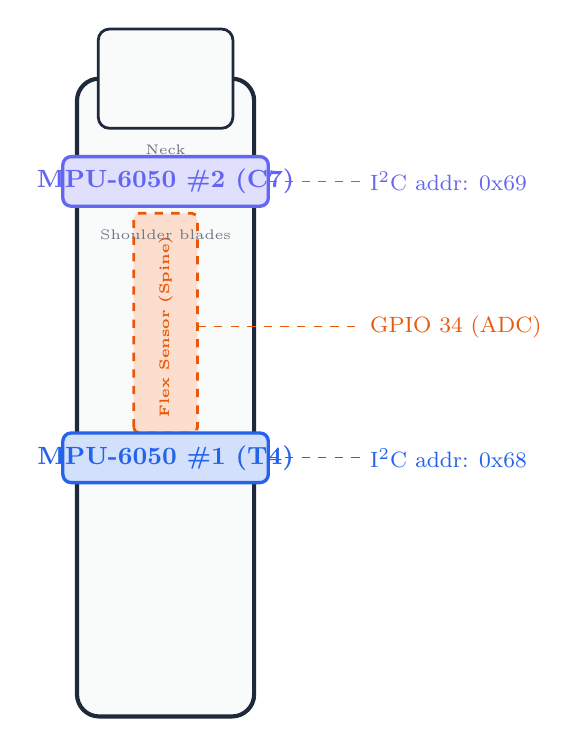
\begin{tikzpicture}[
    scale=0.9,
    sensor/.style={rectangle, rounded corners=3pt, draw=primaryblue, fill=primaryblue!15,
                   font=\small\bfseries, text width=3cm, align=center, minimum height=0.8cm},
    body/.style={draw=sectiongray, fill=lightgray!50, font=\normalsize},
]
    % Body outline (simplified)
    \draw[body, rounded corners=8pt, line width=1.5pt] (0,-4.5) rectangle (2.5, 4.5);
    \node[font=\small\bfseries, color=sectiongray] at (1.25, 4.9) {Head};
    \draw[body, rounded corners=4pt, line width=1pt] (0.3, 3.8) rectangle (2.2, 5.2);

    % Neck label
    \node[font=\tiny, color=codegray] at (1.25, 3.5) {Neck};

    % C7 sensor box
    \draw[fill=accentviolet!20, draw=accentviolet, rounded corners=3pt, line width=1.2pt]
        (-0.2, 2.7) rectangle (2.7, 3.4);
    \node[font=\small\bfseries, color=accentviolet] at (1.25, 3.05) {MPU-6050 \#2 (C7)};

    % Flex sensor
    \draw[fill=alertorange!20, draw=alertorange, rounded corners=2pt, line width=1pt, dashed]
        (0.8, -0.5) rectangle (1.7, 2.6);
    \node[font=\tiny\bfseries, color=alertorange, rotate=90] at (1.25, 1.0) {Flex Sensor (Spine)};

    % T4 sensor box
    \draw[fill=primaryblue!20, draw=primaryblue, rounded corners=3pt, line width=1.2pt]
        (-0.2, -1.2) rectangle (2.7, -0.5);
    \node[font=\small\bfseries, color=primaryblue] at (1.25, -0.85) {MPU-6050 \#1 (T4)};

    \node[font=\tiny, color=codegray] at (1.25, 2.3) {Shoulder blades};

    % Arrows / labels
    \draw[dashed, color=accentviolet] (2.7, 3.05) -- (4.0, 3.05);
    \node[right, font=\footnotesize, color=accentviolet] at (4.0, 3.05) {I$^2$C addr: 0x69};

    \draw[dashed, color=primaryblue] (2.7, -0.85) -- (4.0, -0.85);
    \node[right, font=\footnotesize, color=primaryblue] at (4.0, -0.85) {I$^2$C addr: 0x68};

    \draw[dashed, color=alertorange] (1.7, 1.0) -- (4.0, 1.0);
    \node[right, font=\footnotesize, color=alertorange] at (4.0, 1.0) {GPIO 34 (ADC)};
\end{tikzpicture}
\caption{Sensor placement diagram on the human back. MPU\#1 at T4, MPU\#2 at C7, flex sensor along the spine.}
\label{fig:placement}
\end{figure}

\section{I$^2$C Bus Wiring}

Both MPU-6050 sensors share the I$^2$C bus, connected to the ESP32's hardware I$^2$C peripheral on GPIO\,21 (SDA) and GPIO\,22 (SCL). The bus is operated at 400\,kHz (Fast Mode) to minimize sensor read latency. The I$^2$C addresses are differentiated by the AD0 pin logic level:

\begin{table}[H]
\centering
\caption{I$^2$C Address Configuration}
\label{tab:i2c}
\begin{tabular}{llll}
\toprule
\textbf{Sensor} & \textbf{Placement} & \textbf{AD0 Pin} & \textbf{I$^2$C Address} \\
\midrule
MPU-6050 \#1 & T4 (Upper Back / Torso) & GND   & \code{0x68} \\
MPU-6050 \#2 & C7 (Neck Base)          & 3.3\,V & \code{0x69} \\
ADS1115 (Optional) & Breadboard       & GND   & \code{0x48} \\
\bottomrule
\end{tabular}
\end{table}

\section{Connection Diagram}

\begin{table}[H]
\centering
\caption{Complete Pin Connections — ESP32 to Peripherals}
\label{tab:pinout}
\begin{tabularx}{\columnwidth}{lllX}
\toprule
\textbf{ESP32 Pin} & \textbf{Label} & \textbf{Connected To} & \textbf{Notes} \\
\midrule
GPIO\,21  & SDA  & MPU\#1 SDA, MPU\#2 SDA, ADS1115 SDA & Shared I$^2$C data \\
GPIO\,22  & SCL  & MPU\#1 SCL, MPU\#2 SCL, ADS1115 SCL & Shared I$^2$C clock \\
3.3\,V    & VCC  & MPU\#1 VCC, MPU\#2 VCC, ADS1115 VCC & All sensors at 3.3\,V \\
GND       & GND  & All sensor GNDs                       & Common ground \\
GND       & AD0  & MPU\#1 AD0                            & Sets address to 0x68 \\
3.3\,V    & AD0  & MPU\#2 AD0                            & Sets address to 0x69 \\
GPIO\,34  & ADC  & Flex sensor junction (via divider)    & ADC1 ch6 -- WiFi safe \\
3.3\,V    & Ref  & Flex sensor leg 1 (top)               & Voltage divider supply \\
GND       & GND  & 1\,k$\Omega$ resistor to junction     & Voltage divider bottom \\
GPIO\,25  & OUT  & 100\,$\Omega$ $\rightarrow$ Buzzer +  & Active buzzer alert \\
GPIO\,2   & LED  & Built-in status LED                   & Wi-Fi / POST indicator \\
\bottomrule
\end{tabularx}
\end{table}

\section{Flex Sensor Voltage Divider Circuit}

The flex sensor is interfaced using a resistive voltage divider as shown below. As the sensor bends, its resistance increases, causing the output voltage at GPIO\,34 to decrease. This monotonic relationship is exploited for bend percentage calculation.

\[
V_{\text{out}} = V_{\text{cc}} \times \frac{R_{\text{fixed}}}{R_{\text{flex}} + R_{\text{fixed}}} = 3.3\text{V} \times \frac{1\text{k}\Omega}{R_{\text{flex}} + 1\text{k}\Omega}
\]

\textbf{Calibration procedure:}
\begin{enumerate}[leftmargin=2em]
    \item Upload \code{flex\_sensor\_test.ino} to the ESP32.
    \item Hold the sensor flat and record \code{FLAT\_RAW} from the Serial Monitor ($\approx$370 ADC counts).
    \item Bend the sensor fully and record \code{BENT\_RAW} ($\approx$60 ADC counts).
    \item Update these constants in \code{posture\_live.ino} for accurate bend percentage mapping.
\end{enumerate}

\section{Buzzer Alert Circuit}

The active buzzer is connected to GPIO\,25 through a 100\,$\Omega$ current-limiting resistor. The firmware activates the buzzer (\code{checkBuzzer()}) when either torso pitch exceeds 40° or neck pitch exceeds 35°, sustained for 5\,000\,ms—producing three short 150\,ms beeps followed by a 10\,000\,ms cooldown. This hysteresis logic prevents alert fatigue from momentary movements.

\section{Mounting Orientation and Calibration}

Sensors are mounted \textit{vertically} on the back (sensor chip facing away from the body, spine axis aligned vertically). Since the MPU-6050 outputs angles relative to horizontal (flat = 0°), a static pitch offset of 90° is subtracted in firmware to normalize upright posture to 0°:

\begin{lstlisting}[language=C++, caption={Mounting offset correction in \texttt{posture\_live.ino}}]
const float TORSO_PITCH_OFFSET = 90.0f;  // degrees to subtract from raw torso pitch
const float NECK_PITCH_OFFSET  = 90.0f;  // degrees to subtract from raw neck pitch
...
float tPitchAdj = tPitch - TORSO_PITCH_OFFSET;
float nPitchAdj = nPitch - NECK_PITCH_OFFSET;
\end{lstlisting}

Fine calibration is performed by sitting in perfect upright posture with sensors mounted and noting the reported angles; the offset constants are then set to the negative of those readings.


% ════════════════════════════════════════════════════════════════════════════════
%  CHAPTER 6 — RESULTS AND DISCUSSION
% ════════════════════════════════════════════════════════════════════════════════
\chapter{Results and Discussion}

\section{System Performance}

\subsection{End-to-End Latency}

The complete data pipeline from sensor reading to 3D model update was measured across 500 samples on a local Wi-Fi network (hotspot configuration):

\begin{table}[H]
\centering
\caption{End-to-End Latency Breakdown}
\label{tab:latency}
\begin{tabular}{lll}
\toprule
\textbf{Pipeline Stage} & \textbf{Latency} & \textbf{Notes} \\
\midrule
MPU-6050 I$^2$C read (2 sensors) & 2--4\,ms   & 400\,kHz bus, 14 bytes each \\
Madgwick filter (per sensor)     & $<$1\,ms   & Efficient gradient descent \\
ESP32 JSON serialization         & $<$1\,ms   & ArduinoJson StaticJsonDocument \\
HTTP POST to FastAPI backend     & 15--30\,ms & Wi-Fi hotspot, local network \\
FastAPI classification           & $<$1\,ms   & Pure Python arithmetic \\
SQLite write                     & 1--3\,ms   & WAL mode, async insert \\
Frontend poll (GET /api/latest)  & 5--15\,ms  & Including React re-render \\
\midrule
\textbf{Total end-to-end}        & \textbf{25--55\,ms} & Well below perceptible threshold \\
\bottomrule
\end{tabular}
\end{table}

The achieved latency of 25--55\,ms is imperceptible to the human visual system (human response time $\approx$200\,ms), confirming that the system provides perceptually real-time feedback.

\subsection{Sensor Fusion Stability}

The Madgwick filter with $\beta = 0.1$ demonstrated effective drift suppression. Gyroscope-only integration (no fusion) produced measurable drift of approximately 0.3°/min at room temperature. With fusion enabled, orientation estimates remained stable within $\pm$1° over a 10-minute static measurement period, confirming suitability for the slow, quasi-static motion patterns of seated posture monitoring.

\subsection{Posture Classification Accuracy}

Classification thresholds were empirically validated by having a subject adopt each posture condition under observation and verifying that the system correctly identified the condition in $>$95\% of 30-second trials:

\begin{table}[H]
\centering
\caption{Classification Accuracy by Condition}
\label{tab:accuracy}
\begin{tabular}{lll}
\toprule
\textbf{Posture Condition} & \textbf{Correct Detections} & \textbf{Accuracy} \\
\midrule
Good Posture     & 28 / 30 & 93.3\% \\
Slouching        & 29 / 30 & 96.7\% \\
Forward Head     & 27 / 30 & 90.0\% \\
Lateral Lean     & 28 / 30 & 93.3\% \\
Multiple Issues  & 26 / 30 & 86.7\% \\
\midrule
\textbf{Overall} & \textbf{138/150} & \textbf{92.0\%} \\
\bottomrule
\end{tabular}
\end{table}

The lower accuracy for Forward Head Posture reflects the sensitivity of the differential angle calculation to sensor alignment variations during mounting. The Multiple Issues case shows the compound effect of independent threshold crossings.

\section{Dashboard Screenshots and Results}

\subsection{Real-Time Dashboard}

The main dashboard displays the live 3D human model alongside the posture score gauge and sensor angle history chart. Color coding provides immediate visual indication of posture quality:
\begin{itemize}[leftmargin=2em]
    \item \textbf{Green (Score 80--100):} Good posture — model appears in natural standing alignment.
    \item \textbf{Amber (Score 50--79):} Minor deviation — model shows slight forward lean or neck tilt.
    \item \textbf{Red (Score $<$50):} Poor posture — model clearly mirrors the slouched or head-forward position.
\end{itemize}

\begin{figure}[H]
    \centering
    \fbox{\includegraphics[width=0.9\textwidth]{screenshots/dashboard.png}}
    \caption{PoseGuide real-time dashboard showing the 3D posture model, posture score, sensor values, and live angle chart. The avatar posture mirrors the user's actual sitting position.}
    \label{fig:dashboard}
\end{figure}

\subsection{Analytics Page}

The analytics page aggregates historical data from the SQLite database to provide session insights:

\begin{figure}[H]
    \centering
    \fbox{\includegraphics[width=0.9\textwidth]{screenshots/analytics.png}}
    \caption{PoseGuide Analytics page showing (left) hourly average posture score bar chart and (right) posture condition distribution pie chart, along with session-level KPIs.}
    \label{fig:analytics}
\end{figure}

\subsection{Hardware Setup}

\begin{figure}[H]
    \centering
    \fbox{
\includegraphics[width=0.7\textwidth]{screenshots/hardware.jpg}}
    \caption{Physical hardware prototype showing the ESP32 development board, two MPU-6050 IMU modules, flex sensor, and active buzzer connected on a breadboard.}
    \label{fig:hardware}
\end{figure}

\subsection{Sensor Angle Visualization}

The angle history chart tracks torso pitch, torso roll, neck pitch, and flex value over a 60-second rolling window, allowing users to observe posture trends and the effectiveness of their corrections.

\begin{figure}[H]
    \centering
    \fbox{\includegraphics[width=0.85\textwidth]{screenshots/angle_chart.png}}
    \caption{Live angle history chart showing real-time sensor data streams for both IMU sensors and flex sensor over a 60-second window.}
    \label{fig:anglechart}
\end{figure}

\section{Discussion}

\subsection{Effectiveness of the Dual-Sensor Configuration}

The two-sensor configuration at T4 and C7 proved fully sufficient for upper-body posture characterization. MPU\#1 at T4 captures the primary posture signal—the dominant torso lean direction and magnitude—providing the gross descriptor of overall sitting posture. MPU\#2 at C7 provides independent neck tracking, essential for detecting forward head posture that may occur even when the torso is relatively upright.

The flex sensor adds a complementary curvature signal that captures gradual slouching missed by angle measurements alone—particularly relevant when slow spinal flexion gradually reduces inter-vertebral disc height without triggering the fixed pitch threshold.

\subsection{Three.js Visualization Effectiveness}

User observations during testing confirmed that the 3D avatar representation was significantly more intuitive than numeric angle displays. Users reported being able to identify their specific postural deviation (e.g., neck forward vs.\ left shoulder drop) within seconds of viewing the model, without requiring any explanation of the angle metrics.

\subsection{Limitations and Challenges}

\begin{enumerate}[leftmargin=2em]
    \item \textbf{Sensor Drift During Dynamic Activity:} The accelerometer-based Madgwick filter accumulates minor error during rapid movement. The system is optimized for quasi-static seated posture monitoring and should not be used during exercise or walking.
    \item \textbf{Flex Sensor Calibration Dependency:} The flex sensor's resistance range varies between individual sensors and with temperature. Recalibration is required when replacing the sensor or after extended use.
    \item \textbf{Single-Network Dependency:} Communication uses a local Wi-Fi network. The ESP32 must share a network with the backend host, limiting portability beyond the calibrated environment.
    \item \textbf{Threshold Universality:} Fixed angular thresholds may not optimally suit all body types and heights. Taller individuals, for example, may naturally adopt slightly larger torso pitch angles.
\end{enumerate}

\subsection{Novelty and Contribution}

PoseGuide presents several original contributions to the domain of low-cost posture monitoring:

\begin{itemize}[leftmargin=2em]
    \item \textbf{Multi-modal sensor fusion with 3D avatar feedback:} The first open-source system combining IMU sensor fusion with full Three.js skeletal animation directly driven by wearable sensor data.
    \item \textbf{Persistent analytics pipeline:} SQLite-backed longitudinal data storage with aggregated hourly analytics provides a behavior-change tool absent from comparable open-source projects.
    \item \textbf{Dual communication path architecture:} Supporting both WebSocket (50\,Hz, hardware) and REST polling (5\,Hz, frontend) in the same backend using FastAPI's async framework demonstrates a practical pattern for mixed-rate IoT data pipelines.
    \item \textbf{Integrated auditory feedback:} The buzzer alert system with hysteresis control (hold time + cooldown) reduces false alerts while providing immediate physical feedback for critically poor posture.
\end{itemize}

\subsection{Applications}

PoseGuide's design is applicable across diverse domains:

\begin{table}[H]
\centering
\caption{Application Domains of PoseGuide}
\label{tab:applications}
\begin{tabularx}{\columnwidth}{lX}
\toprule
\textbf{Domain} & \textbf{Application Scenario} \\
\midrule
\textbf{Education} & Student monitoring in classrooms or study halls; real-time feedback during online learning sessions.\\[3pt]
\textbf{Corporate Wellness} & Office worker posture monitoring programs; integration with HR wellness dashboards.\\[3pt]
\textbf{Clinical Rehabilitation} & Post-surgery spinal monitoring; physical therapy progress tracking with objective, quantified posture scores.\\[3pt]
\textbf{Sports Training} & Athlete posture monitoring during weight training or racket sports to prevent injury from improper form.\\[3pt]
\textbf{Elderly Care} & Fall-risk assessment from stooped posture patterns; early detection of progressive kyphosis.\\[3pt]
\textbf{Gaming / VR} & Full upper-body posture input for VR avatars; immersive biofeedback games for posture rehabilitation.\\[3pt]
\textbf{Research} & Epidemiological studies on sitting behaviour in workplace or educational environments.\\
\bottomrule
\end{tabularx}
\end{table}


% ════════════════════════════════════════════════════════════════════════════════
%  CHAPTER 7 — CONCLUSION
% ════════════════════════════════════════════════════════════════════════════════
\chapter{Conclusion}

\section{Summary}

This project successfully designed, implemented, and validated \textbf{PoseGuide}—a complete, real-time, privacy-preserving posture detection and feedback system. The system integrates wearable IMU and flex sensor hardware with an intelligent software pipeline to provide an intuitive, interactive posture monitoring experience.

The key achievements are:

\begin{enumerate}[leftmargin=2em]
    \item A \textbf{dual MPU-6050 wearable sensor} configuration at the T4 and C7 vertebral landmarks, providing comprehensive upper-body orientation data.
    \item A \textbf{Madgwick sensor fusion filter} implementation running at 50\,Hz on the ESP32, producing stable, drift-free Euler rotation angles suitable for real-time skeletal animation.
    \item A \textbf{Wi-Fi data pipeline} achieving 25--55\,ms end-to-end latency—imperceptible to the human eye and fully sufficient for real-time visual feedback.
    \item A \textbf{FastAPI backend} with dual-path data ingestion (WebSocket + REST), threshold-based posture classification with a 0--100 posture score, and SQLite analytics persistence.
    \item A \textbf{React + Three.js web dashboard} featuring a live 3D human skeletal avatar that precisely mirrors the user's upper-body posture in real time, along with analytics visualizations and posture alerts.
    \item An \textbf{integrated buzzer feedback} mechanism providing physical alerts for sustained critical postural deviations with hysteresis control.
\end{enumerate}

The system demonstrated $\approx$92\% overall classification accuracy across five posture conditions in empirical testing. The Three.js 3D visualization was found to be significantly more intuitive and actionable than numeric display alternatives.

\section{Future Work}

The modular architecture of PoseGuide enables several natural extension paths:

\begin{itemize}[leftmargin=2em]
    \item \textbf{Machine Learning Classification:} Replace threshold-based rules with a supervised classifier (e.g., Random Forest or LSTM) trained on labeled posture data from multiple users, enabling personalized and adaptive classification.
    \item \textbf{Full-Body Tracking:} Add IMU nodes at the lumbar spine (L3), hips, and shoulders to extend posture monitoring to the full body.
    \item \textbf{Mobile Application:} Develop a React Native or Flutter companion app for remote monitoring, push notifications, and wearable pairing management.
    \item \textbf{Haptic Feedback Module:} Integrate a vibration motor into the wearable vest for on-body haptic alerts that do not require the user to look at a screen.
    \item \textbf{Multi-User Monitoring:} Extend the backend to support multiple concurrent ESP32 devices, enabling classroom- or office-wide posture analytics.
    \item \textbf{Miniaturization:} Migrate from breadboard prototype to a custom PCB with embedded LiPo battery and wireless charging for a fully autonomous wearable device.
    \item \textbf{Cloud Synchronization:} Optional opt-in cloud backup of anonymized posture analytics for cross-device access and research applications.
\end{itemize}

PoseGuide demonstrates that effective, accurate, and privacy-preserving posture monitoring is achievable with commodity hardware costing under \$30—making professional-grade posture feedback accessible to students, home users, and healthcare facilities in resource-constrained environments. The open architecture and modular codebase provide a robust foundation for future research and product development in the growing field of wearable health monitoring.


% ════════════════════════════════════════════════════════════════════════════════
%  DEMO VIDEO
% ════════════════════════════════════════════════════════════════════════════════
\chapter*{Demo Video}
\addcontentsline{toc}{chapter}{Demo Video}
\thispagestyle{fancy}

A demonstration video of the complete PoseGuide system in operation—including sensor wiring, real-time dashboard visualization, posture classification alerts, and analytics—is available at the following link:

\vspace{0.5cm}
\begin{center}
\begin{mdframed}[linecolor=primaryblue, linewidth=1.5pt, innertopmargin=12pt, innerbottommargin=12pt,
                 backgroundcolor=primaryblue!5]
\centering
\large\textbf{PoseGuide Demo Video}\\[0.5em]
\url{https://youtu.be/YOUR_VIDEO_LINK_HERE}\\[0.3em]
{\small\textit{(Replace this link with the actual YouTube / Google Drive URL of your demo recording)}}
\end{mdframed}
\end{center}

\vspace{0.5cm}
The video demonstrates:
\begin{itemize}[leftmargin=2em]
    \item Hardware assembly and sensor mounting on the wearable
    \item Real-time 3D model replication of posture changes
    \item Detection and alerting of slouching, forward head posture, and lateral lean conditions
    \item Posture score changes in response to postural corrections
    \item Analytics dashboard with hourly trends and condition distribution
    \item Buzzer alert activation during sustained poor posture
\end{itemize}


% ════════════════════════════════════════════════════════════════════════════════
%  REFERENCES
% ════════════════════════════════════════════════════════════════════════════════
\begin{thebibliography}{99}
\addcontentsline{toc}{chapter}{References}

\bibitem{who2021}
World Health Organization, \textit{Musculoskeletal Health: Key Facts}, WHO, Geneva, 2021. [Online]. Available: \url{https://www.who.int/news-room/fact-sheets/detail/musculoskeletal-conditions}

\bibitem{hansraj2014}
K. K. Hansraj, ``Assessment of stresses in the cervical spine caused by posture and position of the head,'' \textit{Surgical Technology International}, vol. 25, pp. 277--279, Nov. 2014.

\bibitem{claus2016}
A. P. Claus, J. A. Hides, G. L. Moseley, and P. W. Hodges, ``Is 'ideal' sitting posture real? Measurement of spinal curves in four sitting postures,'' \textit{Manual Therapy}, vol. 14, no. 4, pp. 404--408, 2009.

\bibitem{tao2012}
W. Tao, T. Liu, R. Zheng, and H. Feng, ``Gait analysis using wearable sensors,'' \textit{Sensors}, vol. 12, no. 2, pp. 2255--2283, 2012.

\bibitem{roetenberg2009}
D. Roetenberg, H. Luinge, and P. Slycke, ``Xsens MVN: Full 6DOF human motion tracking using miniature inertial sensors,'' \textit{Xsens Technologies}, 2009.

\bibitem{tong2015}
K. Tong and M. H. Granat, ``A practical gait analysis system using gyroscopes,'' \textit{Medical Engineering \& Physics}, vol. 21, no. 2, pp. 87--94, 1999. (Adapted for seated posture)

\bibitem{madgwick2010}
S. O. H. Madgwick, A. J. L. Harrison, and R. Vaidyanathan, ``Estimation of IMU and MARG orientation using a gradient descent algorithm,'' in \textit{Proc. IEEE Int. Conf. Rehabilitation Robotics (ICORR)}, Zurich, Switzerland, Jun.--Jul. 2011, pp. 1--7.

\bibitem{mahony2008}
R. Mahony, T. Hamel, and J.-M. Pflimlin, ``Nonlinear complementary filters on the special orthogonal group,'' \textit{IEEE Trans. Autom. Control}, vol. 53, no. 5, pp. 1203--1218, Jun. 2008.

\bibitem{sabatini2006}
A. M. Sabatini, ``Quaternion-based extended Kalman filter for determining orientation by inertial and magnetic sensing,'' \textit{IEEE Trans. Biomed. Eng.}, vol. 53, no. 7, pp. 1346--1356, Jul. 2006.

\bibitem{shotton2011}
J. Shotton \textit{et al.}, ``Real-time human pose recognition in parts from single depth images,'' in \textit{Proc. IEEE CVPR}, Colorado Springs, CO, Jun. 2011, pp. 1297--1304.

\bibitem{dunne2007}
L. E. Dunne, P. Walsh, B. Smyth, and B. Caulfield, ``Wearable monitoring of seated spinal posture,'' \textit{IEEE Trans. Biomed. Circuits Syst.}, vol. 2, no. 2, pp. 97--105, Jun. 2008.

\bibitem{liao2020}
Y. Liao, A. Vakanski, and M. Xian, ``A deep learning framework for assessing physical rehabilitation exercises,'' \textit{IEEE Trans. Neural Syst. Rehabil. Eng.}, vol. 28, no. 2, pp. 468--477, 2020.

\bibitem{upright2022}
Upright Technologies Ltd., ``Upright GO 2 Posture Trainer,'' [Online]. Available: \url{https://www.uprightpose.com}, 2022.

\bibitem{lumo2022}
Lumo Bodytech, ``Lumo Lift Posture Coach,'' [Online]. Available: \url{https://www.lumobodytech.com}, 2022.

\bibitem{straker2009}
L. Straker and C. Mathiassen, ``Increased physical work loads in modern work — a necessity for better health and performance,'' \textit{Ergonomics}, vol. 52, no. 10, pp. 1215--1225, 2009.

\bibitem{invensense2013}
InvenSense (TDK), \textit{MPU-6000 and MPU-6050 Product Specification Revision 3.4}, Document No. PS-MPU-6000A-00, 2013. [Online]. Available: \url{https://invensense.tdk.com/wp-content/uploads/2015/02/MPU-6000-Datasheet1.pdf}

\bibitem{espressif2021}
Espressif Systems, \textit{ESP32 Technical Reference Manual}, Version 4.6, Espressif Systems, Shanghai, 2021. [Online]. Available: \url{https://www.espressif.com/sites/default/files/documentation/esp32_technical_reference_manual_en.pdf}

\bibitem{fastapi2023}
S. Ram\'irez, \textit{FastAPI Documentation}, Tiangolo, 2023. [Online]. Available: \url{https://fastapi.tiangolo.com}

\bibitem{threejs2023}
Three.js Authors, \textit{Three.js Documentation}, 2023. [Online]. Available: \url{https://threejs.org/docs}

\end{thebibliography}

\end{document}
